\documentclass{standalone}
\usepackage{tikz}
\usetikzlibrary{patterns, positioning}


\begin{document}
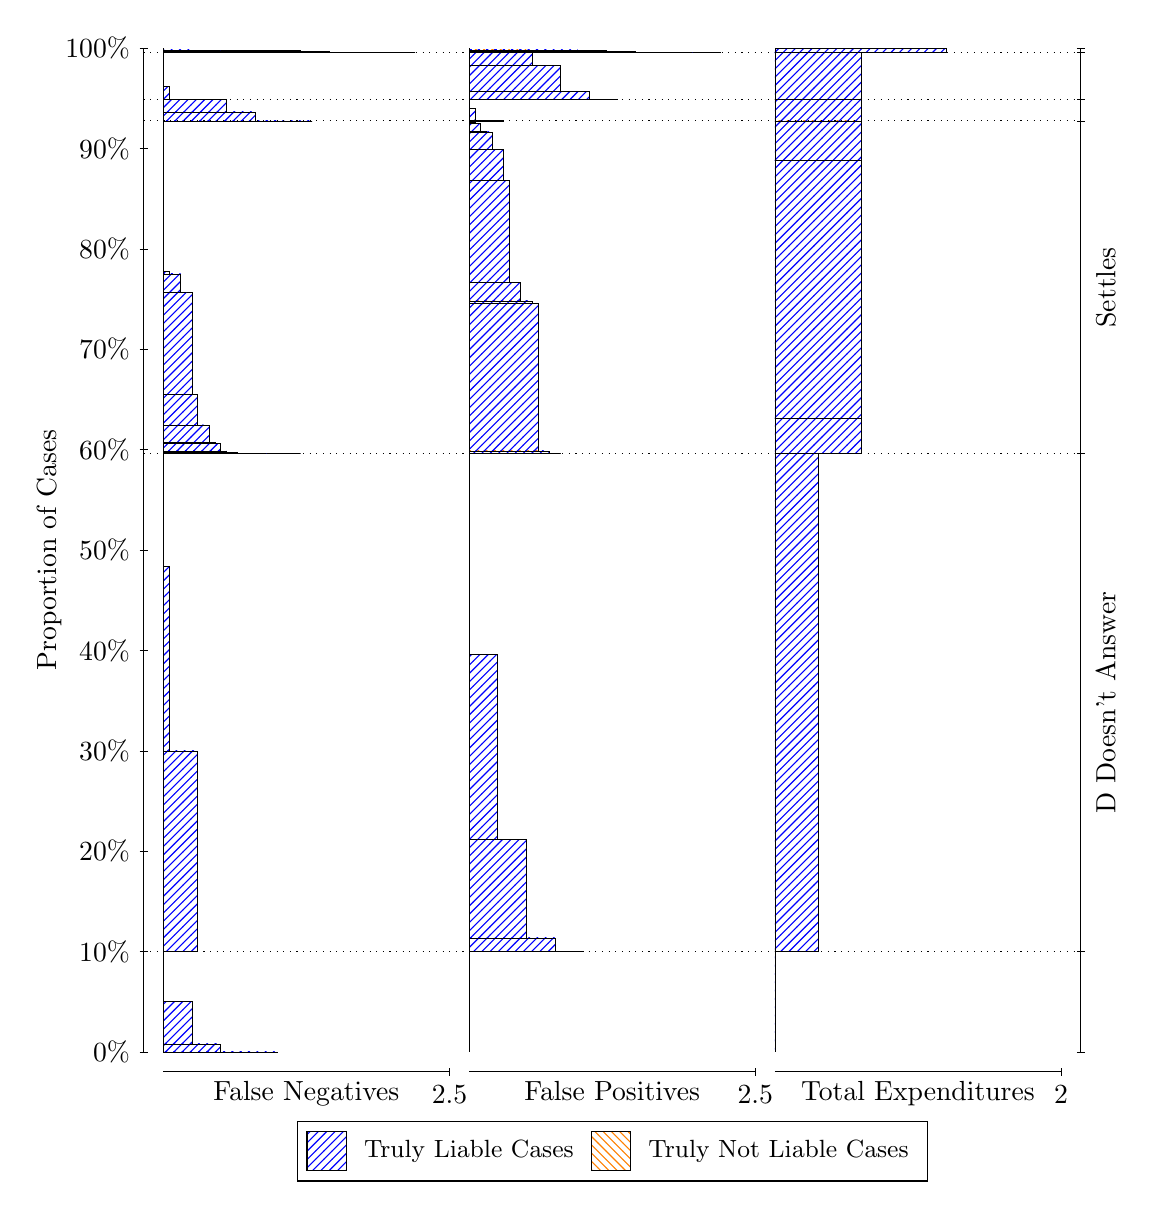
\begin{tikzpicture}
\draw[black, very thin] (1.5,1.75) -- (1.5,14.5);
\node[rotate=90, text=black, anchor=center] at (0.3, 8.125) {Proportion of Cases};
\draw[black, very thin] (1.45,1.75) -- (1.55,1.75);
\node[text=black, anchor=east] at (1.45, 1.75) {0\%};
\draw[black, very thin] (1.45,3.025) -- (1.55,3.025);
\node[text=black, anchor=east] at (1.45, 3.025) {10\%};
\draw[black, very thin] (1.45,4.3) -- (1.55,4.3);
\node[text=black, anchor=east] at (1.45, 4.3) {20\%};
\draw[black, very thin] (1.45,5.575) -- (1.55,5.575);
\node[text=black, anchor=east] at (1.45, 5.575) {30\%};
\draw[black, very thin] (1.45,6.85) -- (1.55,6.85);
\node[text=black, anchor=east] at (1.45, 6.85) {40\%};
\draw[black, very thin] (1.45,8.125) -- (1.55,8.125);
\node[text=black, anchor=east] at (1.45, 8.125) {50\%};
\draw[black, very thin] (1.45,9.4) -- (1.55,9.4);
\node[text=black, anchor=east] at (1.45, 9.4) {60\%};
\draw[black, very thin] (1.45,10.675) -- (1.55,10.675);
\node[text=black, anchor=east] at (1.45, 10.675) {70\%};
\draw[black, very thin] (1.45,11.95) -- (1.55,11.95);
\node[text=black, anchor=east] at (1.45, 11.95) {80\%};
\draw[black, very thin] (1.45,13.225) -- (1.55,13.225);
\node[text=black, anchor=east] at (1.45, 13.225) {90\%};
\draw[black, very thin] (1.45,14.5) -- (1.55,14.5);
\node[text=black, anchor=east] at (1.45, 14.5) {100\%};

\draw[black, very thin] (13.4,1.75) -- (13.4,14.5);
\draw[black, very thin] (13.35,1.75) -- (13.45,1.75);
\node[anchor=west] at (13.35, 1.75) {};
\draw[black, very thin] (13.35,3.0247) -- (13.45,3.0247);
\node[anchor=west] at (13.35, 3.0247) {};
\draw[black, very thin] (13.35,9.348) -- (13.45,9.348);
\node[anchor=west] at (13.35, 9.348) {};
\draw[black, very thin] (13.35,13.575) -- (13.45,13.575);
\node[anchor=west] at (13.35, 13.575) {};
\draw[black, very thin] (13.35,13.846) -- (13.45,13.846);
\node[anchor=west] at (13.35, 13.846) {};
\draw[black, very thin] (13.35,14.448) -- (13.45,14.448);
\node[anchor=west] at (13.35, 14.448) {};
\draw[black, very thin] (13.35,14.5) -- (13.45,14.5);
\node[anchor=west] at (13.35, 14.5) {};

\draw[black, very thin, pattern color=blue, pattern=north east lines] (1.75,1.75) rectangle (3.2033,1.75);
\draw[black, very thin, pattern color=blue, pattern=north east lines] (1.75,1.75) rectangle (2.84,1.7509);
\draw[black, very thin, pattern color=blue, pattern=north east lines] (1.75,1.7509) rectangle (2.4767,1.852);
\draw[black, very thin, pattern color=blue, pattern=north east lines] (1.75,1.852) rectangle (2.1133,2.3882);
\draw[black, very thin, pattern color=orange, pattern=north west lines] (1.75,2.3882) rectangle (1.75,2.3882);
\draw[black, very thin, pattern color=blue, pattern=north east lines] (1.75,2.3882) rectangle (1.75,3.0247);
\draw[black, very thin, pattern color=blue, pattern=north east lines] (1.75,3.0247) rectangle (2.186,5.5726);
\draw[black, very thin, pattern color=blue, pattern=north east lines] (1.75,5.5726) rectangle (1.8227,7.9231);
\draw[black, very thin, pattern color=orange, pattern=north west lines] (1.75,7.9231) rectangle (1.75,7.9231);
\draw[black, very thin, pattern color=blue, pattern=north east lines] (1.75,7.9231) rectangle (1.75,9.348);
\draw[black, very thin, pattern color=blue, pattern=north east lines] (1.75,9.348) rectangle (3.494,9.348);
\draw[black, very thin, pattern color=blue, pattern=north east lines] (1.75,9.348) rectangle (3.3487,9.348);
\draw[black, very thin, pattern color=blue, pattern=north east lines] (1.75,9.348) rectangle (3.2033,9.348);
\draw[black, very thin, pattern color=blue, pattern=north east lines] (1.75,9.348) rectangle (3.1307,9.348);
\draw[black, very thin, pattern color=blue, pattern=north east lines] (1.75,9.348) rectangle (3.058,9.348);
\draw[black, very thin, pattern color=blue, pattern=north east lines] (1.75,9.348) rectangle (2.9853,9.348);
\draw[black, very thin, pattern color=blue, pattern=north east lines] (1.75,9.348) rectangle (2.9127,9.348);
\draw[black, very thin, pattern color=blue, pattern=north east lines] (1.75,9.348) rectangle (2.84,9.349);
\draw[black, very thin, pattern color=blue, pattern=north east lines] (1.75,9.349) rectangle (2.7673,9.3543);
\draw[black, very thin, pattern color=blue, pattern=north east lines] (1.75,9.3543) rectangle (2.6947,9.3609);
\draw[black, very thin, pattern color=blue, pattern=north east lines] (1.75,9.3609) rectangle (2.622,9.3626);
\draw[black, very thin, pattern color=blue, pattern=north east lines] (1.75,9.3626) rectangle (2.5493,9.3827);
\draw[black, very thin, pattern color=blue, pattern=north east lines] (1.75,9.3827) rectangle (2.4767,9.4805);
\draw[black, very thin, pattern color=blue, pattern=north east lines] (1.75,9.4805) rectangle (2.404,9.4874);
\draw[black, very thin, pattern color=blue, pattern=north east lines] (1.75,9.4874) rectangle (2.3313,9.712);
\draw[black, very thin, pattern color=blue, pattern=north east lines] (1.75,9.712) rectangle (2.2587,9.7137);
\draw[black, very thin, pattern color=blue, pattern=north east lines] (1.75,9.7137) rectangle (2.186,10.105);
\draw[black, very thin, pattern color=blue, pattern=north east lines] (1.75,10.105) rectangle (2.1133,11.396);
\draw[black, very thin, pattern color=blue, pattern=north east lines] (1.75,11.396) rectangle (2.0407,11.396);
\draw[black, very thin, pattern color=blue, pattern=north east lines] (1.75,11.396) rectangle (1.968,11.633);
\draw[black, very thin, pattern color=blue, pattern=north east lines] (1.75,11.633) rectangle (1.8953,11.633);
\draw[black, very thin, pattern color=blue, pattern=north east lines] (1.75,11.633) rectangle (1.8227,11.667);
\draw[black, very thin, pattern color=orange, pattern=north west lines] (1.75,11.667) rectangle (1.75,11.667);
\draw[black, very thin, pattern color=blue, pattern=north east lines] (1.75,11.667) rectangle (1.75,13.575);
\draw[black, very thin, pattern color=blue, pattern=north east lines] (1.75,13.575) rectangle (3.6393,13.575);
\draw[black, very thin, pattern color=blue, pattern=north east lines] (1.75,13.575) rectangle (3.276,13.575);
\draw[black, very thin, pattern color=blue, pattern=north east lines] (1.75,13.575) rectangle (2.9127,13.689);
\draw[black, very thin, pattern color=blue, pattern=north east lines] (1.75,13.689) rectangle (2.5493,13.843);
\draw[black, very thin, pattern color=blue, pattern=north east lines] (1.75,13.843) rectangle (2.186,13.846);
\draw[black, very thin, pattern color=orange, pattern=north west lines] (1.75,13.846) rectangle (1.75,13.846);
\draw[black, very thin, pattern color=blue, pattern=north east lines] (1.75,13.846) rectangle (2.186,13.848);
\draw[black, very thin, pattern color=blue, pattern=north east lines] (1.75,13.848) rectangle (1.8227,14.017);
\draw[black, very thin, pattern color=orange, pattern=north west lines] (1.75,14.017) rectangle (1.75,14.017);
\draw[black, very thin, pattern color=blue, pattern=north east lines] (1.75,14.017) rectangle (1.75,14.448);
\draw[black, very thin, pattern color=blue, pattern=north east lines] (1.75,14.448) rectangle (4.9473,14.448);
\draw[black, very thin, pattern color=blue, pattern=north east lines] (1.75,14.448) rectangle (4.584,14.448);
\draw[black, very thin, pattern color=blue, pattern=north east lines] (1.75,14.448) rectangle (4.2207,14.449);
\draw[black, very thin, pattern color=blue, pattern=north east lines] (1.75,14.449) rectangle (3.8573,14.458);
\draw[black, very thin, pattern color=blue, pattern=north east lines] (1.75,14.458) rectangle (3.494,14.472);
\draw[black, very thin, pattern color=blue, pattern=north east lines] (1.75,14.472) rectangle (3.1307,14.473);
\draw[black, very thin, pattern color=blue, pattern=north east lines] (1.75,14.473) rectangle (2.84,14.473);
\draw[black, very thin, pattern color=blue, pattern=north east lines] (1.75,14.473) rectangle (2.7673,14.473);
\draw[black, very thin, pattern color=blue, pattern=north east lines] (1.75,14.473) rectangle (2.4767,14.473);
\draw[black, very thin, pattern color=blue, pattern=north east lines] (1.75,14.473) rectangle (2.1133,14.476);
\draw[black, very thin, pattern color=orange, pattern=north west lines] (1.75,14.476) rectangle (1.75,14.476);
\draw[black, very thin, pattern color=blue, pattern=north east lines] (1.75,14.476) rectangle (1.75,14.5);
\draw[black, very thin, pattern color=orange, pattern=north west lines] (5.6333,1.75) rectangle (5.6333,1.75);
\draw[black, very thin, pattern color=blue, pattern=north east lines] (5.6333,1.75) rectangle (5.6333,3.0247);
\draw[black, very thin, pattern color=orange, pattern=north west lines] (5.6333,3.0247) rectangle (7.0867,3.0247);
\draw[black, very thin, pattern color=blue, pattern=north east lines] (5.6333,3.0247) rectangle (7.0867,3.0264);
\draw[black, very thin, pattern color=blue, pattern=north east lines] (5.6333,3.0264) rectangle (6.7233,3.1977);
\draw[black, very thin, pattern color=blue, pattern=north east lines] (5.6333,3.1977) rectangle (6.36,4.4496);
\draw[black, very thin, pattern color=blue, pattern=north east lines] (5.6333,4.4496) rectangle (5.9967,6.8001);
\draw[black, very thin, pattern color=blue, pattern=north east lines] (5.6333,6.8001) rectangle (5.6333,9.348);
\draw[black, very thin, pattern color=orange, pattern=north west lines] (5.6333,9.348) rectangle (6.796,9.348);
\draw[black, very thin, pattern color=blue, pattern=north east lines] (5.6333,9.348) rectangle (6.796,9.348);
\draw[black, very thin, pattern color=orange, pattern=north west lines] (5.6333,9.348) rectangle (6.6507,9.348);
\draw[black, very thin, pattern color=blue, pattern=north east lines] (5.6333,9.348) rectangle (6.6507,9.385);
\draw[black, very thin, pattern color=orange, pattern=north west lines] (5.6333,9.385) rectangle (6.5053,9.385);
\draw[black, very thin, pattern color=blue, pattern=north east lines] (5.6333,9.385) rectangle (6.5053,11.256);
\draw[black, very thin, pattern color=blue, pattern=north east lines] (5.6333,11.256) rectangle (6.4327,11.29);
\draw[black, very thin, pattern color=orange, pattern=north west lines] (5.6333,11.29) rectangle (6.36,11.29);
\draw[black, very thin, pattern color=blue, pattern=north east lines] (5.6333,11.29) rectangle (6.36,11.29);
\draw[black, very thin, pattern color=blue, pattern=north east lines] (5.6333,11.29) rectangle (6.2873,11.527);
\draw[black, very thin, pattern color=orange, pattern=north west lines] (5.6333,11.527) rectangle (6.2147,11.527);
\draw[black, very thin, pattern color=blue, pattern=north east lines] (5.6333,11.527) rectangle (6.2147,11.527);
\draw[black, very thin, pattern color=blue, pattern=north east lines] (5.6333,11.527) rectangle (6.142,12.818);
\draw[black, very thin, pattern color=blue, pattern=north east lines] (5.6333,12.818) rectangle (6.0693,13.209);
\draw[black, very thin, pattern color=blue, pattern=north east lines] (5.6333,13.209) rectangle (5.9967,13.211);
\draw[black, very thin, pattern color=blue, pattern=north east lines] (5.6333,13.211) rectangle (5.924,13.436);
\draw[black, very thin, pattern color=blue, pattern=north east lines] (5.6333,13.436) rectangle (5.8513,13.442);
\draw[black, very thin, pattern color=blue, pattern=north east lines] (5.6333,13.442) rectangle (5.7787,13.54);
\draw[black, very thin, pattern color=blue, pattern=north east lines] (5.6333,13.54) rectangle (5.706,13.56);
\draw[black, very thin, pattern color=blue, pattern=north east lines] (5.6333,13.56) rectangle (5.6333,13.575);
\draw[black, very thin, pattern color=orange, pattern=north west lines] (5.6333,13.575) rectangle (6.0693,13.575);
\draw[black, very thin, pattern color=blue, pattern=north east lines] (5.6333,13.575) rectangle (6.0693,13.577);
\draw[black, very thin, pattern color=blue, pattern=north east lines] (5.6333,13.577) rectangle (5.706,13.731);
\draw[black, very thin, pattern color=blue, pattern=north east lines] (5.6333,13.731) rectangle (5.6333,13.846);
\draw[black, very thin, pattern color=orange, pattern=north west lines] (5.6333,13.846) rectangle (7.5227,13.846);
\draw[black, very thin, pattern color=blue, pattern=north east lines] (5.6333,13.846) rectangle (7.5227,13.846);
\draw[black, very thin, pattern color=blue, pattern=north east lines] (5.6333,13.846) rectangle (7.1593,13.945);
\draw[black, very thin, pattern color=blue, pattern=north east lines] (5.6333,13.945) rectangle (6.796,14.276);
\draw[black, very thin, pattern color=blue, pattern=north east lines] (5.6333,14.276) rectangle (6.4327,14.446);
\draw[black, very thin, pattern color=blue, pattern=north east lines] (5.6333,14.446) rectangle (6.0693,14.448);
\draw[black, very thin, pattern color=orange, pattern=north west lines] (5.6333,14.448) rectangle (8.8307,14.448);
\draw[black, very thin, pattern color=blue, pattern=north east lines] (5.6333,14.448) rectangle (8.8307,14.448);
\draw[black, very thin, pattern color=blue, pattern=north east lines] (5.6333,14.448) rectangle (8.4673,14.448);
\draw[black, very thin, pattern color=orange, pattern=north west lines] (5.6333,14.448) rectangle (8.4673,14.448);
\draw[black, very thin, pattern color=blue, pattern=north east lines] (5.6333,14.448) rectangle (8.4673,14.448);
\draw[black, very thin, pattern color=blue, pattern=north east lines] (5.6333,14.448) rectangle (8.104,14.449);
\draw[black, very thin, pattern color=orange, pattern=north west lines] (5.6333,14.449) rectangle (8.104,14.449);
\draw[black, very thin, pattern color=blue, pattern=north east lines] (5.6333,14.449) rectangle (8.104,14.449);
\draw[black, very thin, pattern color=blue, pattern=north east lines] (5.6333,14.449) rectangle (7.7407,14.449);
\draw[black, very thin, pattern color=orange, pattern=north west lines] (5.6333,14.449) rectangle (7.7407,14.449);
\draw[black, very thin, pattern color=blue, pattern=north east lines] (5.6333,14.449) rectangle (7.7407,14.46);
\draw[black, very thin, pattern color=blue, pattern=north east lines] (5.6333,14.46) rectangle (7.3773,14.46);
\draw[black, very thin, pattern color=blue, pattern=north east lines] (5.6333,14.46) rectangle (7.3773,14.472);
\draw[black, very thin, pattern color=blue, pattern=north east lines] (5.6333,14.472) rectangle (7.014,14.475);
\draw[black, very thin, pattern color=blue, pattern=north east lines] (5.6333,14.475) rectangle (6.6507,14.475);
\draw[black, very thin, pattern color=orange, pattern=north west lines] (5.6333,14.475) rectangle (6.36,14.475);
\draw[black, very thin, pattern color=blue, pattern=north east lines] (5.6333,14.475) rectangle (6.36,14.475);
\draw[black, very thin, pattern color=blue, pattern=north east lines] (5.6333,14.475) rectangle (6.2873,14.475);
\draw[black, very thin, pattern color=orange, pattern=north west lines] (5.6333,14.475) rectangle (5.9967,14.475);
\draw[black, very thin, pattern color=blue, pattern=north east lines] (5.6333,14.475) rectangle (5.9967,14.476);
\draw[black, very thin, pattern color=orange, pattern=north west lines] (5.6333,14.476) rectangle (5.6333,14.476);
\draw[black, very thin, pattern color=blue, pattern=north east lines] (5.6333,14.476) rectangle (5.6333,14.5);
\draw[black, very thin, pattern color=orange, pattern=north west lines] (9.5167,1.75) rectangle (9.5167,1.75);
\draw[black, very thin, pattern color=blue, pattern=north east lines] (9.5167,1.75) rectangle (9.5167,3.0247);
\draw[black, very thin, pattern color=orange, pattern=north west lines] (9.5167,3.0247) rectangle (10.062,3.0247);
\draw[black, very thin, pattern color=blue, pattern=north east lines] (9.5167,3.0247) rectangle (10.062,9.348);
\draw[black, very thin, pattern color=orange, pattern=north west lines] (9.5167,9.348) rectangle (10.607,9.348);
\draw[black, very thin, pattern color=blue, pattern=north east lines] (9.5167,9.348) rectangle (10.607,9.7935);
\draw[black, very thin, pattern color=orange, pattern=north west lines] (9.5167,9.7935) rectangle (10.607,9.7935);
\draw[black, very thin, pattern color=blue, pattern=north east lines] (9.5167,9.7935) rectangle (10.607,13.07);
\draw[black, very thin, pattern color=orange, pattern=north west lines] (9.5167,13.07) rectangle (10.607,13.07);
\draw[black, very thin, pattern color=blue, pattern=north east lines] (9.5167,13.07) rectangle (10.607,13.575);
\draw[black, very thin, pattern color=orange, pattern=north west lines] (9.5167,13.575) rectangle (10.607,13.575);
\draw[black, very thin, pattern color=blue, pattern=north east lines] (9.5167,13.575) rectangle (10.607,13.846);
\draw[black, very thin, pattern color=orange, pattern=north west lines] (9.5167,13.846) rectangle (10.607,13.846);
\draw[black, very thin, pattern color=blue, pattern=north east lines] (9.5167,13.846) rectangle (10.607,14.448);
\draw[black, very thin, pattern color=orange, pattern=north west lines] (9.5167,14.448) rectangle (11.697,14.448);
\draw[black, very thin, pattern color=blue, pattern=north east lines] (9.5167,14.448) rectangle (11.697,14.449);
\draw[black, very thin, pattern color=orange, pattern=north west lines] (9.5167,14.449) rectangle (11.697,14.449);
\draw[black, very thin, pattern color=blue, pattern=north east lines] (9.5167,14.449) rectangle (11.697,14.5);
\draw[black, dotted] (1.5,3.0247) -- (13.4,3.0247);
\draw[black, dotted] (1.5,9.348) -- (13.4,9.348);
\draw[black, dotted] (1.5,13.575) -- (13.4,13.575);
\draw[black, dotted] (1.5,13.846) -- (13.4,13.846);
\draw[black, dotted] (1.5,14.448) -- (13.4,14.448);
\draw[black, very thin] (1.75,1.5) -- (5.3833,1.5);
\node[text=black, anchor=north] at (3.5667, 1.5) {False Negatives};
\draw[black, very thin] (5.3833,1.45) -- (5.3833,1.55);
\node[text=black, anchor=north] at (5.3833, 1.45) {2.5};

\draw[black, very thin] (5.6333,1.5) -- (9.2667,1.5);
\node[text=black, anchor=north] at (7.45, 1.5) {False Positives};
\draw[black, very thin] (9.2667,1.45) -- (9.2667,1.55);
\node[text=black, anchor=north] at (9.2667, 1.45) {2.5};

\draw[black, very thin] (9.5167,1.5) -- (13.15,1.5);
\node[text=black, anchor=north] at (11.333, 1.5) {Total Expenditures};
\draw[black, very thin] (13.15,1.45) -- (13.15,1.55);
\node[text=black, anchor=north] at (13.15, 1.45) {2};


\node[text=black, centered, rotate=90] at (13.72, 6.1864) {D Doesn't Answer};
\node[text=black, centered, rotate=90] at (13.72, 11.461) {Settles};




\draw (7.449999999999999,1.5) node[draw=none] (baseCoordinate) {};
\begin{scope}[align=center]
        \matrix[scale=0.5, draw=black, below=0.5cm of baseCoordinate, nodes={draw}, column sep=0.1cm]{
            \node[rectangle, draw, minimum width=0.5cm, minimum height=0.5cm, pattern color=blue, pattern=north east lines] {}; &
            \node[draw=none, font=\small, text=black] (B) {Truly Liable Cases}; &
            \node[rectangle, draw, minimum width=0.5cm, minimum height=0.5cm, pattern color=orange, pattern=north west lines] {}; &
            \node[draw=none, font=\small, text=black] (B) {Truly Not Liable Cases}; \\
            };
\end{scope}

\end{tikzpicture}
\end{document}